\section{Structure from Motion}\label{SfM}

Mithilfe des "Structure from Motion"-Verfahrens (SfM) können dreidimensionale Informationen aus einer Reihe von zweidimensionalen Bildern rekonstruiert werden. SfM basiert auf der Triangulation von Punkten, die in verschiedenen Bildern sichtbar sind, um die Positionen der Sensoren und der Punkte in der Szene zu bestimmen. 

Dieses Verfahren ist die Grundlage vieler AR-Technologien und wird in verschiedenen AR-Frameworks in verbesserter bzw. abgewandelter Form (z.B. SLAM, siehe Kapitel \ref{SLAM}) eingesetzt. Daher ist es wichtig, die grundlegenden Schritte und Algorithmen zu verstehen, die bei der Rekonstruktion von dreidimensionalen Szenen verwendet werden. (\cite{doerner2022virtual})

\subsection{Feature Detection und Matching}

Bei der Feature Detection bzw. beim Feature Maching werden Merkmale in verschiedenen Bildern identifiziert und korrespondierende Merkmale gefunden. Dieser Schritt ist entscheidend, um die Bewegung der Kamera (Tracking) und die 3D-Struktur der Szene zu bestimmen. Es gibt verschiedene Algorithmen, die für das Erkennen und Nachverfolgen von Feature-Punkten verwendet werden können, wie z. B. SIFT (Scale-Invariant Feature Transform), SURF (Speeded-Up Robust Features) oder ORB (Oriented FAST and Rotated BRIEF). Diese Algorithmen setzen sich grundsätzlich aus drei Teilen zusammen:

\begin{enumerate}
    \item Feature Detector oder Keypoint Detector
    \item Feature Descriptor
    \item Feature Matching Algorithm
\end{enumerate}

Der Feature Detector identifiziert charakteristische Punkte im Bild, die sich durch hohe Kontraste oder markante Strukturen auszeichnen. Diese Punkte, auch als Keypoints bezeichnet, dienen als Referenz für spätere Berechnungen. Anschließend erstellt der Feature Descriptor eine numerische Beschreibung für jedes erkannte Merkmal, um sie über mehrere Bilder hinweg vergleichbar zu machen. Diese Deskriptoren bestehen in der Regel aus Vektoren, die die Helligkeitsverteilung um den jeweiligen Feature-Punkt erfassen. Schließlich vergleicht der Feature Matching Algorithmus die Deskriptoren aus verschiedenen Bildern, um korrespondierende Merkmale zu finden, die wiederum zur Schätzung der Kamerabewegung genutzt werden.

Ein besonders effizienter und robuster Algorithmus ist ORB, der auf den Methoden FAST (Features from Accelerated Segment Test) und BRIEF (Binary Robust Independent Elementary Features) basiert. Der FAST-Algorithmus erkennt Punkte mit starken Helligkeitsänderungen, indem er benachbarte Pixel in einem Kreis um den zu prüfenden Pixel vergleicht. Übersteigt die Anzahl der signifikant helleren oder dunkleren Pixel einen bestimmten Schwellenwert, wird der Punkt als Feature identifiziert. Anschließend berechnet BRIEF für jedes erkannte Feature binäre Deskriptoren, indem zufällig gewählte Pixelpaare innerhalb der Umgebung des Feature-Punkts verglichen werden. Die resultierenden binären Deskriptoren sind besonders effizient in der Berechnung und Speicherung. Um die erkannten Merkmale schnell und zuverlässig zuzuordnen, kommt die Fast Library for Approximate Nearest Neighbors (FLANN) zum Einsatz, die eine leistungsstarke Methode zur Suche nach korrespondierenden Features bietet.

Neben klassischen Verfahren wie ORB gewinnen Deep-Learning-Modelle zunehmend an Bedeutung für das Feature Matching. Besonders Convolutional Neural Networks (CNNs) und Transformer-Modelle liefern vielversprechende Ergebnisse. Ein Beispiel hierfür ist XFeat (Accelerated Features), ein optimiertes neuronales Netzwerk, das die Merkmalsextraktion beschleunigt. Auch OmniGlue, eine Kombination aus CNNs und Transformer-Modellen, setzt neue Maßstäbe in der robusten und anpassungsfähigen Feature-Matching-Strategie. Diese modernen Ansätze bieten oft eine höhere Genauigkeit und Stabilität, insbesondere in komplexen Szenen oder bei stark variierenden Lichtverhältnissen.

\subsection{Camera Pose Estimation}

Die Schätzung der Kameraposition ist ein essenzieller Schritt in der SfM-Pipeline, da sie die Position und Orientierung der Kamera in jedem Bild bestimmt. Diese Informationen sind entscheidend für die Rekonstruktion der 3D-Struktur der Szene und die Bestimmung der extrinsischen Kameraparameter.

Geht man davon aus, dass die intrinsischen Parameter der Kamera bekannt sind und mehrere Bilder mit korrespondierenden Punkten vorliegen, kann die Kameraposition mithilfe der Essential Matrix \(E\) berechnet werden. Diese Matrix beschreibt die geometrische Beziehung zwischen zwei Bildern und ermöglicht die Bestimmung von Rotation und Translation der Kamera. Die grundlegende Bedingung für die Berechnung der extrinsischen Parameter lautet:

\begin{equation}
x'^T E x = 0
\end{equation}

Diese Gleichung beschreibt die Epipolargeometrie, wobei \( x \) und \( x' \) die korrespondierenden Punkte in den beiden Bildern darstellen. Die Essential Matrix kann durch den Five-Point-Algorithmus geschätzt werden, der im kalibrierten Fall mindestens fünf korrespondierende Punkte benötigt, um eine eindeutige Lösung zu liefern.

Sobald die Essential Matrix bestimmt wurde, kann sie mithilfe der Singulärwertzerlegung (SVD) in die Rotationsmatrix \( R \) und die Translationsmatrix \( t \) der Kamera zerlegt werden:

\begin{equation}
E = R [t]_x
\end{equation}

Diese Zerlegung erlaubt es, die Bewegung der Kamera zwischen den Bildern präzise zu bestimmen.

\subsection{Dreidimensionale Rekonstruktion}

Die dreidimensionale Rekonstruktion einer Szene überführt die zweidimensionalen Bilddaten einer Kamera in ein 3D-Modell. Dabei werden sowohl die Kameraparameter als auch die Translation und Rotation der Kamera sowie die korrespondierenden Feature-Punkte aus dem Feature Matching verwendet, um die Positionen der Punkte im Raum zu berechnen und so eine präzise 3D-Darstellung der Szene zu erstellen.

Ein zentraler Schritt in der 3D-Rekonstruktion ist die Triangulation, bei der die kartesischen Koordinaten eines Feature-Punktes im Weltkoordinatensystem ermittelt werden. Ein einfaches Verfahren zur Bestimmung dieser Koordinaten besteht darin, den 3D-Strahlen zu folgen, die von den Kamerazentren \( c_j \) in die Richtungen \( \hat{v_j} \) verlaufen. Der gesuchte Punkt \( p_0 \) ist derjenige, der sich im minimalen Abstand zu allen Strahlen befindet. Die Richtungen \( \hat{v_j} \) werden durch die Transformation der 2D-Bildpunkte mittels der Kameramatrizen beschrieben. Der Punkt \( p_0 \) wird dabei durch Minimierung der quadratischen Abstände zwischen den Strahlen und dem Punkt berechnet.

\begin{figure}
    \centering
    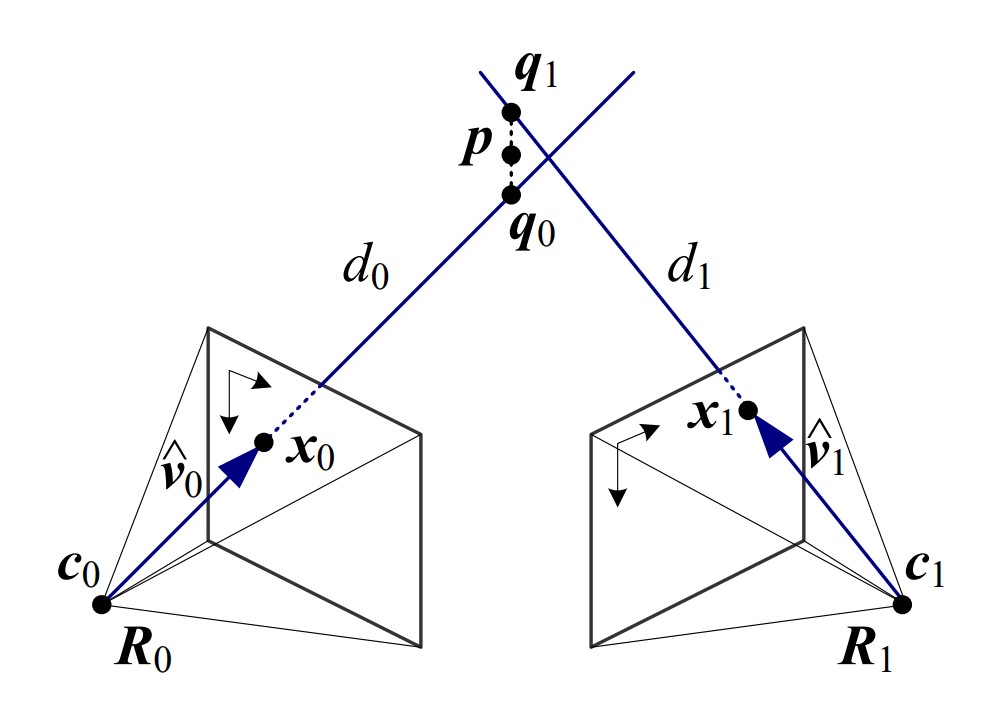
\includegraphics[width=.5\textwidth]{Triangulation}
    \caption{Dreidimensionale Triangulation mit zwei Bildern\label{fig:Triangulation}}\par
\end{figure}

Abbildung \ref{fig:Triangulation} zeigt die grafische Darstellung der Triangulation eines Punktes im dreidimensionalen Raum. Mathematisch wird dieser Prozess durch die folgende Gleichung beschrieben:

\[
p = \left( \sum_j \left( I - \hat{v_j} \hat{v_j}^T \right) \right)^{-1} \left( \sum_j \left( I - \hat{v_j} \hat{v_j}^T \right) c_j \right)
\]

Das Ergebnis der Triangulation ist eine sogenannte Punktwolke (Point Cloud), die die 3D-Struktur der Szene abbildet. Diese Punktwolke kann anschließend weiterverarbeitet werden, um ein detailliertes 3D-Modell der Szene zu erstellen. Ein wichtiger Schritt in dieser Weiterverarbeitung ist die Oberflächenrekonstruktion (Plane Detection), bei der die Punktwolke in Flächen unterteilt wird, um die Oberflächen von Objekten im Raum zu bestimmen. Zur Durchführung der Oberflächenrekonstruktion wird häufig der RANSAC-Algorithmus (Random Sample Consensus) eingesetzt. Dieser Algorithmus erkennt Ausreißer in den Daten und schätzt die Flächen anhand der verbleibenden, konsistenten Punkte.

\begin{figure}
    \centering
    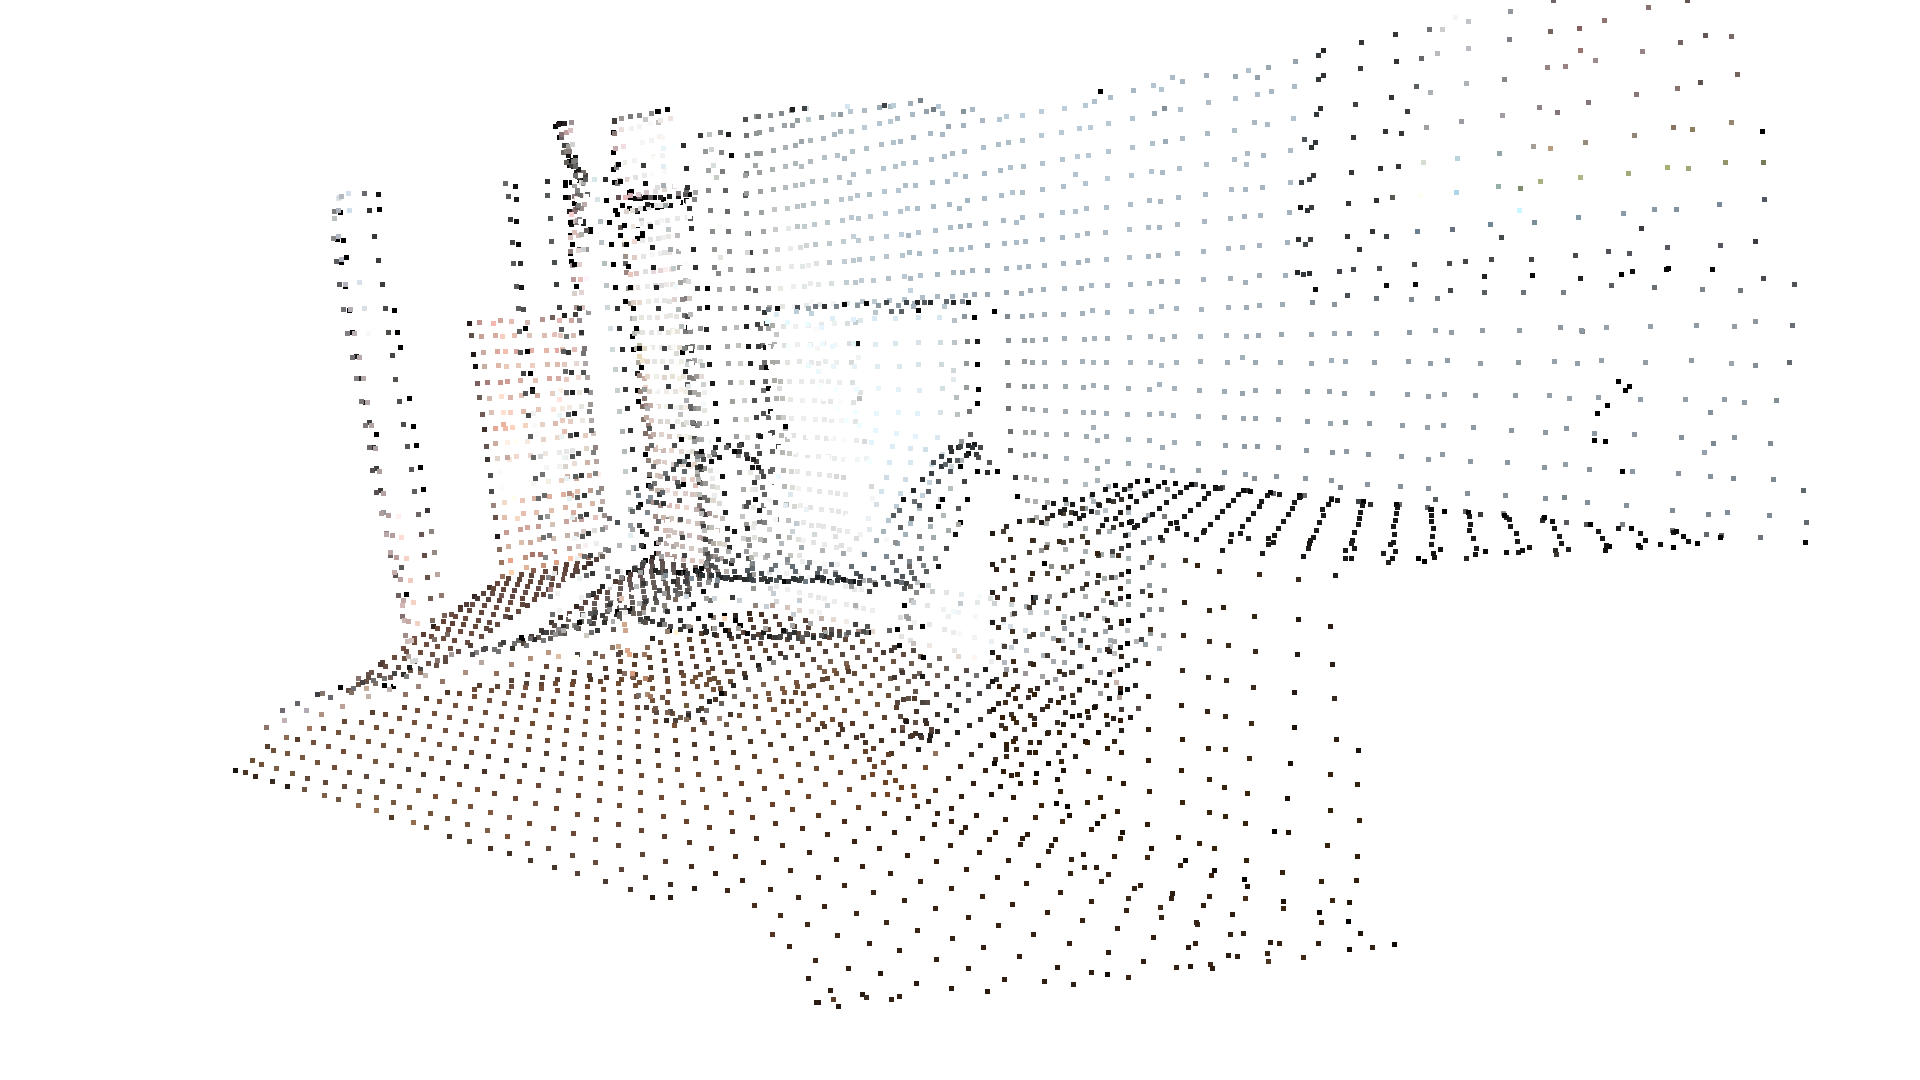
\includegraphics[ width=.5\textwidth ]{PointCloud}
    \caption{Beispiel einer drei-dimensionalen Point-Cloud-Rekonstruktion\label{fig:PointCloud}}\par
\end{figure}

\subsection{Bundle Adjustment}

Der Bundle Adjustment ist ein Optimierungsverfahren, das verwendet wird, um die Kamerapositionen und die 3D-Struktur der Szene zu verfeinern. Dabei werden die Fehler zwischen den projizierten 3D-Punkten und den tatsächlichen 2D-Punkten minimiert, um die bestmögliche Schätzung der Kamerapositionen und der 3D-Struktur zu erhalten. Der Bundle Adjustment ist ein iterativer Prozess, der normalerweise auf der nicht-linearen Optimierung basiert. Es gibt verschiedene Algorithmen zur Bundle Adjustment, wie z. B. die Levenberg-Marquardt-Methode oder die Gauss-Newton-Methode.